\section{Regristrasi Oracle Apex}

Pada tahap ini yaitu regristrasi pada website oracle express online sampai akan terbuka halaman pertama aplikasi oracle expresss, yang harus dibutuhkan pertama kali saat menggunakan Oracle Apex Online dengan membuat akun terlebih dahulu membuat workspace dan lain-lain.

hal-hal yang dilakukan saat regristrasi yaitu :

\begin{itemize}
        
        \begin{figure}[!htbp]
        \item[1]Masuk Pada Halaman Oracle APEX ONLINE yaitu https://apex.oracle.com/en/, pada halaman pertama tampilan akan seperti ini, pada bagian title terdapat tulisan yang mengartikan Membuat Aplikasi ini dapat memudahkan skala, keamanan penggunaan aplikasi, dan dengan cepat akan terbuat, langsung saja klik pada tombol sign in, lihat pada Gambar 2.1.
        \begin{center}
        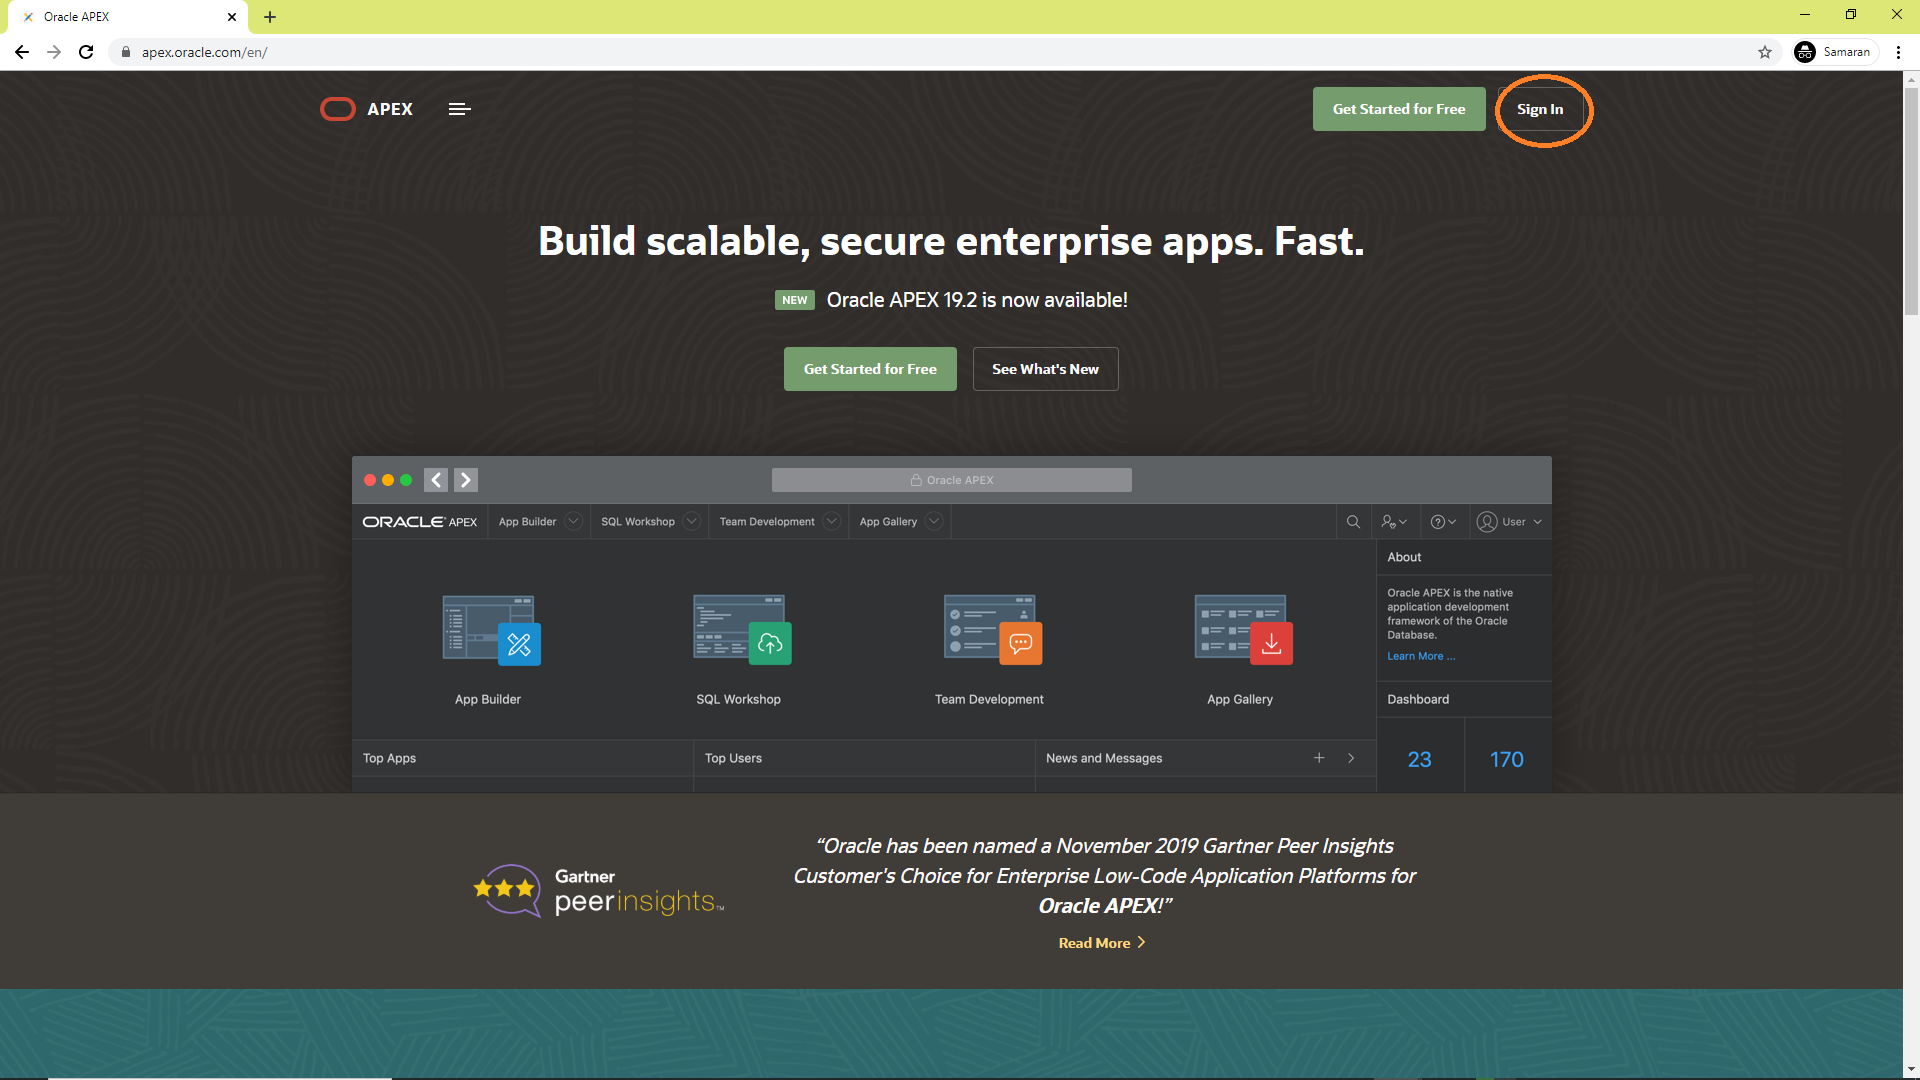
\includegraphics[scale=0.23]{figures/1.png}
        \caption{\textit{Halaman APEX.ORACLE.COM}}
        \end{center}
        \end{figure}
        
        
        \begin{figure}[!htbp]
        \item[2]Pada Halaman Login Klik Request a Workspace, karena kita belum mempunyai akun kita akan regristrasi terlebih dahulu, pada form yang di gambar yaitu form untuk login untuk memasuki halaman aplikasi kita yang saat kita buat nanti,  lihat pada Gambar 2.2.
        \begin{center}
        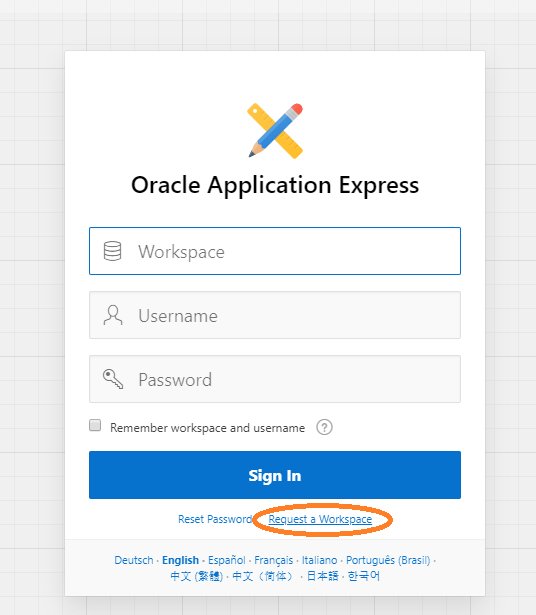
\includegraphics[scale=0.5]{figures/2.png}
        \caption{\textit{Req Workspace}}
        \end{center}
        \end{figure}
        
        \begin{figure}[!htbp]
        \item[3]Isikan data diri anda dengan benar ,lihat pada Gambar 2.3, First Name = Isikan Nama Depan Anda, Last Name = Isikan Nama Belakang Anda, Email = Isikan Email Anda (Wajib karena saat mengisi semua form regristrasi nanti akan diberikan notifikasi melalui email, Workspace = Nama Proyek yang akan dibuat.
        \begin{center}
        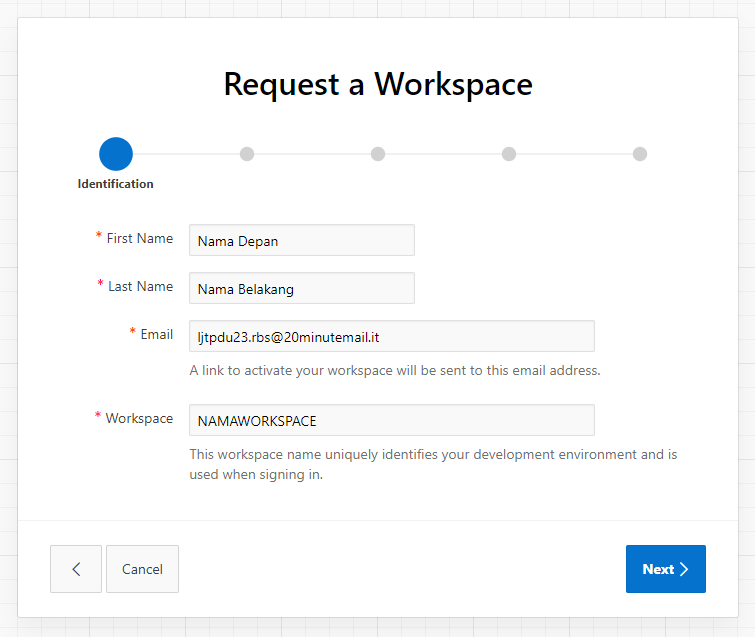
\includegraphics[scale=0.5]{figures/3.png}
        \caption{\textit{Req Workspace2}}
        \end{center}
        \end{figure}
        
        \begin{figure}[!htbp]
        \item[4]Berikut adalah Survey dimana oracle akan memastikan anda menggunakan dengan baik aplikasi yang akan anda kembangkan , pertama oracle akan menanyakan "Apakah anda pengguna baru Oracle Application Express?", dan yang kedua "Apakah kamu mempunyai plan menggunakan proyek ini untuk universitas atau pelatihan ?", isilah data data berikut seperti Gambar 2.4.
        \begin{center}
        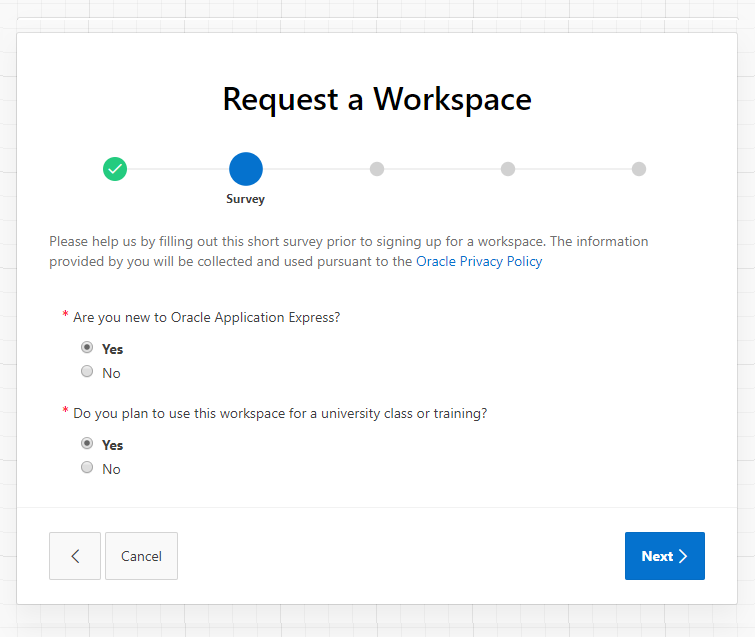
\includegraphics[scale=0.5]{figures/4.png}
        \caption{\textit{Req Workspace3}}
        \end{center}
        \end{figure}
        
        \begin{figure}[!htbp]
        \item[5]Form berikut adalah form justification atau pembenaran, atau melihat apakah anda robot atau tidak oracle akan menanyakan "Mengapa anda ingin meminta akses serfis ini ?" isikan form berikut bebas dengan kata-kata yang anda sukai, lihat pada Gambar 2.5.
        \begin{center}
        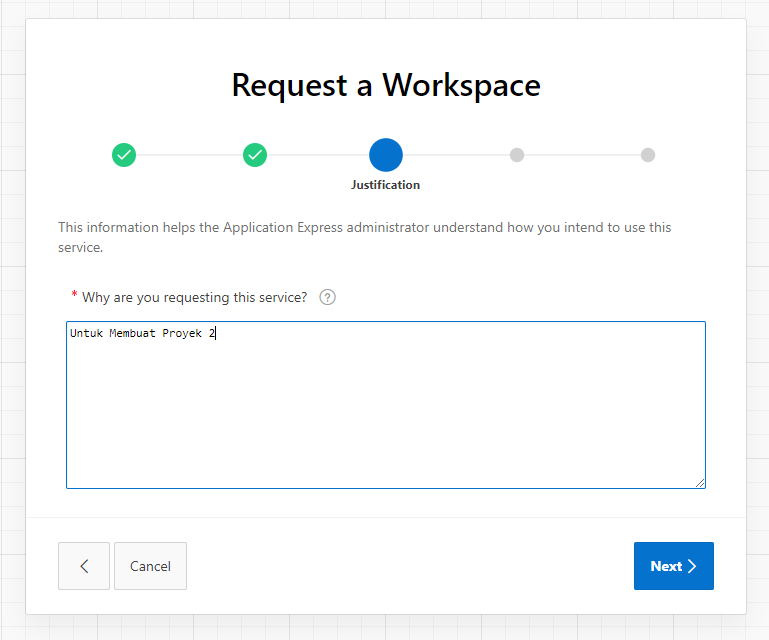
\includegraphics[scale=0.5]{figures/5.png}
        \caption{\textit{Req Workspace4}}
        \end{center}
        \end{figure}
        
        \begin{figure}[!htbp]
        \item[6]Berikut adalah step form Persetujuan, oracle akan menanyakan apakah kamu akan menyetujui semua persetujuan menggunakan aplikasi, jika anda setuju centang "I accept the terms", lihat pada Gambar 2.6.
        \begin{center}
        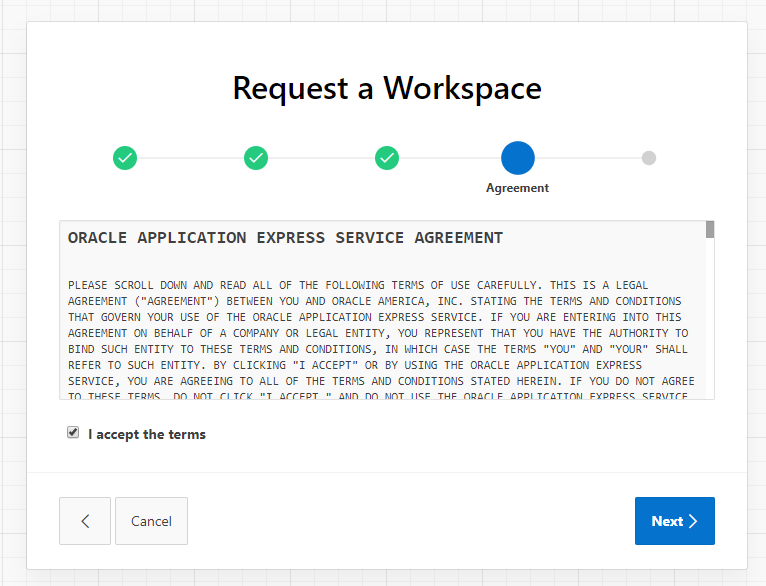
\includegraphics[scale=0.5]{figures/6.png}
        \caption{\textit{Req Workspace5}}
        \end{center}
        \end{figure}

        \begin{figure}[!htbp]
        \item[7]Berikut adalah step form Konfirmasi apakah data yang anda inputkan sudah benar jika semua sudah benar klik Submit Request, lihat pada Gambar 2.7.
        \begin{center}
        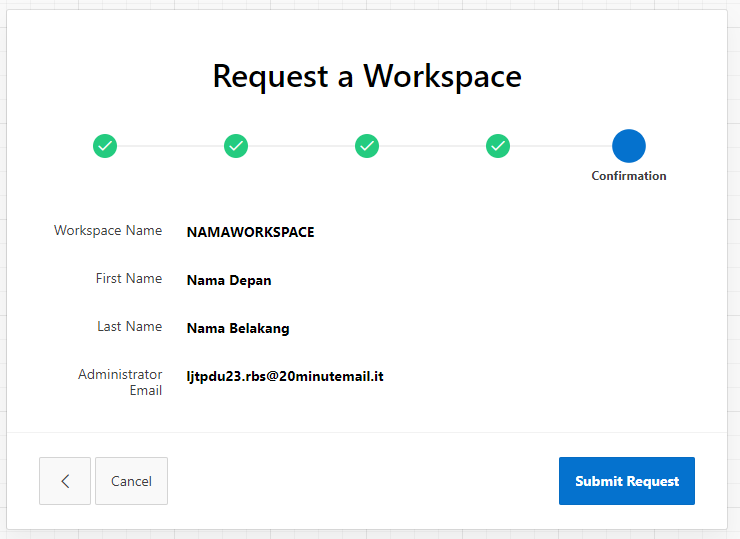
\includegraphics[scale=0.5]{figures/7.png}
        \caption{\textit{Req Workspace6}}
        \end{center}
        \end{figure}
        
        \begin{figure}[!htbp]
        \item[8]Permintaan membuat projek telah terkirim, anda akan menerima email yang anda inputkan saat mengisi form Regristrasi tadi, segera cek email anda, kalau belum di terima biasanya akan ada waktu interval 0-15 menit, karena oracle akan mengidentifikasi form yang anda inputkan tadi,lihat pada Gambar 2.8.
        \begin{center}
        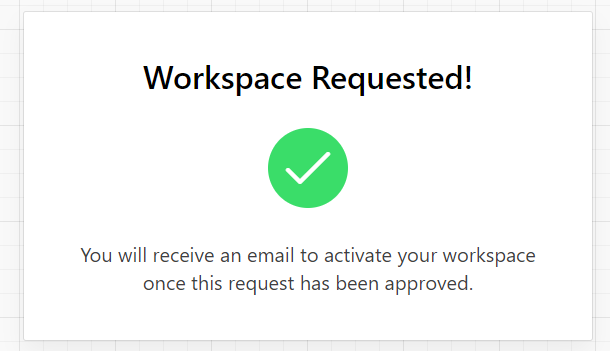
\includegraphics[scale=0.5]{figures/8.png}
        \caption{\textit{Req Workspace7}}
        \end{center}
        \end{figure}
        
        \begin{figure}[!htbp]
        \item[9]Saat anda menerima email seperti berikut dengan data data yang anda inputkan pada form tadi seperti Workspace dan Username, lalu anda akan menerima link untuk environment, setelah semua dirasa benar klik tombol "Create Workspace", lihat pada Gambar 2.9.
        \begin{center}
        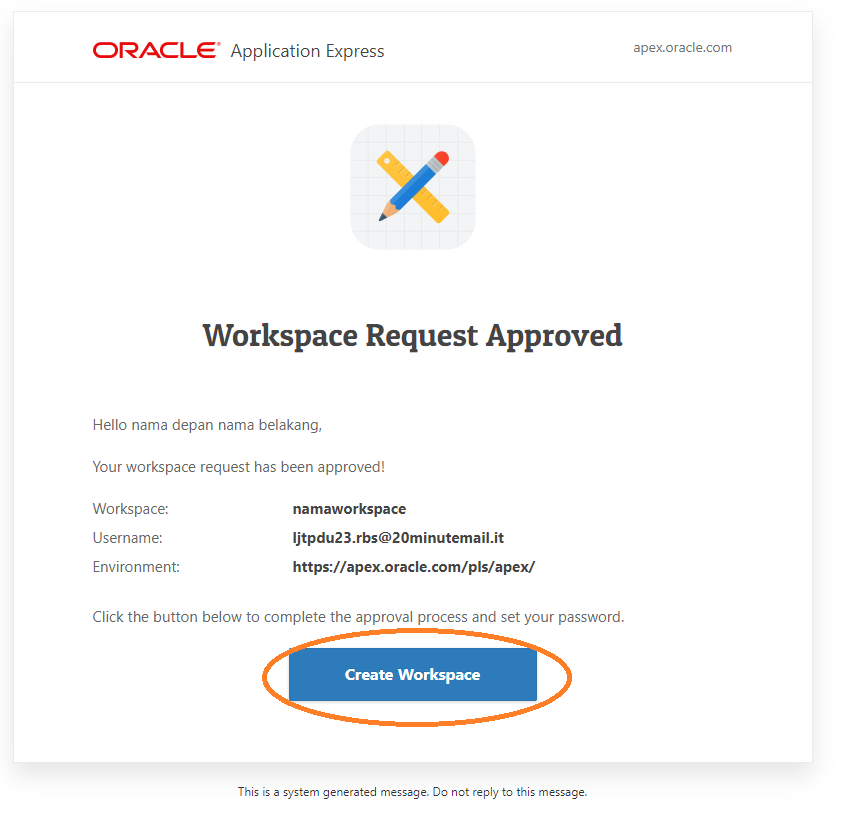
\includegraphics[scale=0.5]{figures/9.png}
        \caption{\textit{Cek Email}}
        \end{center}
        \end{figure}
        
        \begin{figure}[!htbp]
        \item[10]Selamat Workspace anda telah dibuat ! , anda akan diberitahu notifikasi tersebut , lalu selanjutnya anda lakukan Continue to Sign In Screen, lihat pada Gambar 2.10.
        \begin{center}
        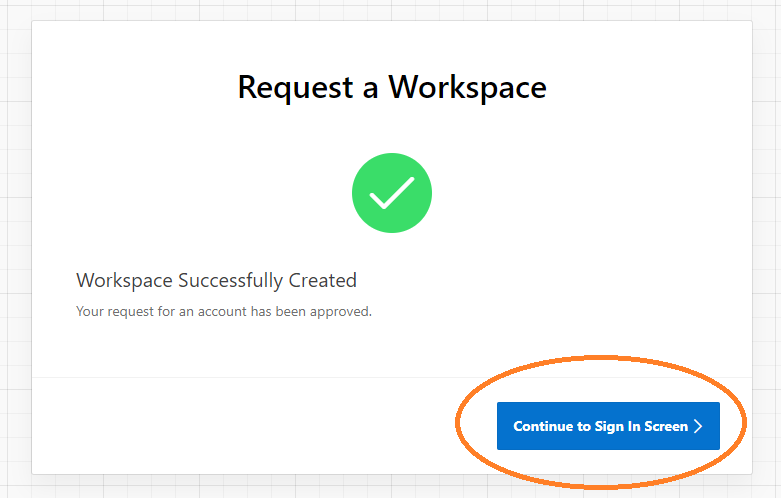
\includegraphics[scale=0.5]{figures/10.png}
        \caption{\textit{Continue to Sign In Screen}}
        \end{center}
        \end{figure}
        
        \begin{figure}[!htbp]
        \item[11]Lalu anda akan dialihkan pada halaman untuk mengganti password untuk workspace anda, Masukkan password anda yg diinginkan dan konfirmasi password ke 2 secara benar, lalu klik Apply Changes, lihat pada Gambar 2.11.
        \begin{center}
        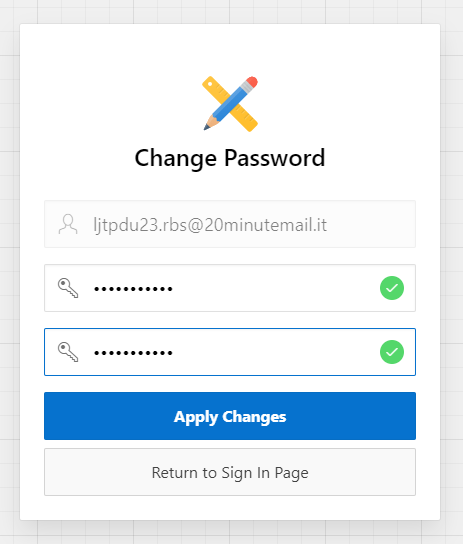
\includegraphics[scale=0.5]{figures/11.png}
        \caption{\textit{Masukan Password}}
        \end{center}
        \end{figure}
        
        \begin{figure}[!htbp]
        \item[12]Jika sudah membuat password, anda akan dialihkan pada halaman utama Aplikasi Oracle Apex, yang dimana anda akan membuat aplikasi, lihat pada Gambar 2.12.
        
        \begin{itemize}
            \item App Builder = Untuk membuat dan mengelola aplikasi web, pastikan database sudah ada.
            \item SQL Workshop = Untuk membuat dan mengelola Database, setiap informasi biasanya tertuju pada SQL Workspace.
            \item  Team Development = adalah aplikasi bawaan yang dikelola oleh APEX, namun kita tidak akan menggunakan fitur ini.
            \item App Gallery = Untuk membuat aplikasi yang sudah ada atau sudah jadi untuk dimasukkan ke workspace kita, namun kita tidak akan menggunakan fitur ini.
        \end{itemize}
        \par Pada panel sebelah kiri anda akan dijelaskan tentang apa itu Oracle Apex, Dashboard yang berisi berapa banyak Aplikasi anda, Tables berapa banyak jumlah tabel.
        \par Lalu ada Site Specific Task yaitu website yang akan mengalihkan pada suatu guide atau yang membahas  tentang Oracle APEX,
        \par Lalu Resources, adalah halaman komunitas-komunitas yang telah diremiskan oleh Oracle Apex.
        \par Tab Social, adalah halaman social Oracle Apex yang sering dijumpai.
        \begin{center}
        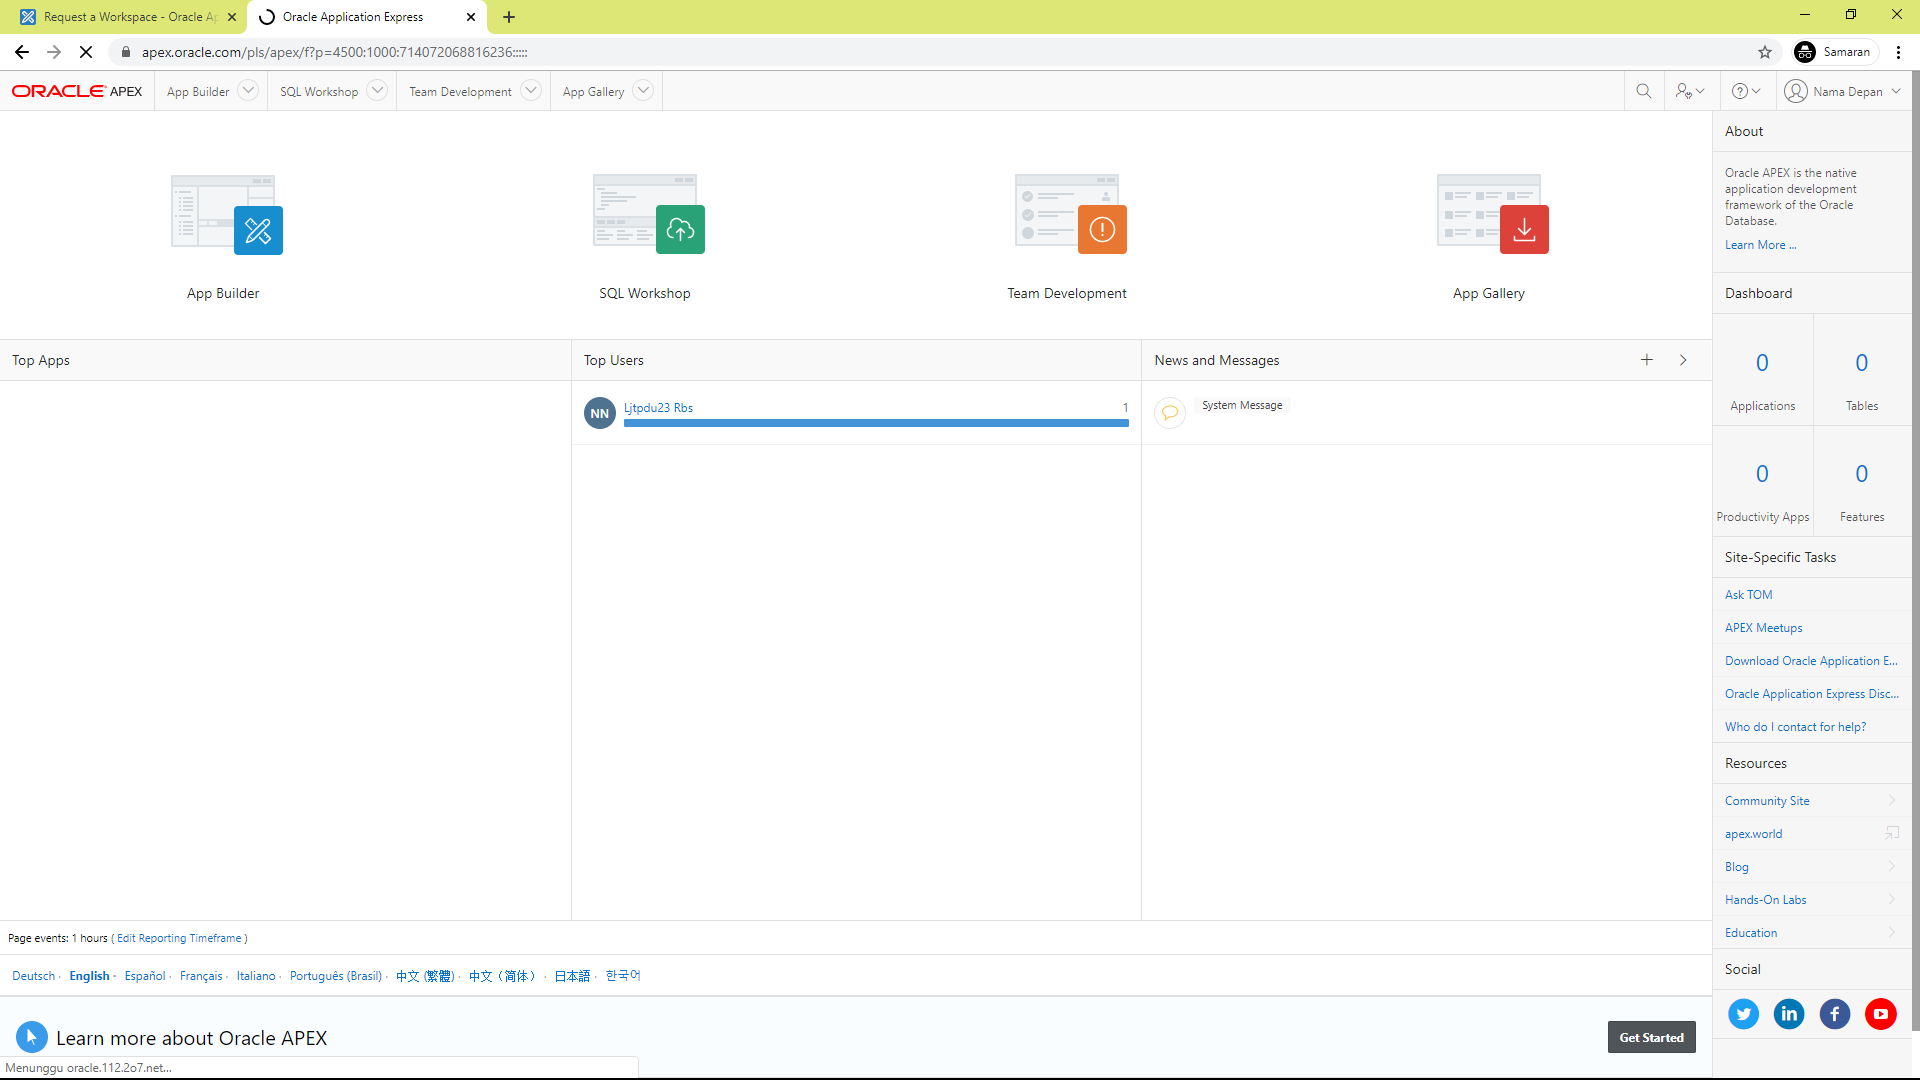
\includegraphics[scale=0.23]{figures/12.png}
        \caption{\textit{Halaman Utama Apex}}
        \end{center}
        \end{figure}
\end{itemize}